\section{Esperanza Condicionada}

\begin{ejercicio}
    Sea $X$ una variable aleatoria que se distribuye uniformemente en el intervalo $\left]0,1\right[$. Comprobar si las variables aleatorias $X$ y $|\nicefrac{1}{2}-X|$ son incorreladas.

    % // TODO: Incorreladas?
\end{ejercicio}

\begin{ejercicio}
    Calcular las curvas de regresión y las razones de correlación para las siguientes distribuciones, comentando los resultados.
    \begin{enumerate}
        \item Considerar las distribución conjunta $(X,Y)$ con función de masa de probabilidad dada por:
        \begin{equation*}
            \begin{array}{c|ccc||c}
                X\setminus Y & 10 & 15 & 20 & \\
                \hline
                1 & 0 & \nicefrac{2}{6} & 0 & \nicefrac{2}{6}\\
                2 & \nicefrac{1}{6} & 0 & 0 & \nicefrac{1}{6}\\
                3 & 0 & 0 & \nicefrac{3}{6} & \nicefrac{3}{6}\\
                \hline \hline
                & \nicefrac{1}{6} & \nicefrac{2}{6} & \nicefrac{3}{6} & 1
            \end{array}
        \end{equation*}

        Tras haber calculado las distribuciones marginales, calculamos ahora las distribuciones condicionadas.
        La siguiente tabla muestra la distribución condicionada de $Y$ dado $X$, $P[Y = y\mid X = x]$:
        \begin{equation*}
            \begin{array}{c|ccc}
                X\setminus Y & 10 & 15 & 20 \\
                \hline
                1 & 0 & 1 & 0\\
                2 & 1 & 0 & 0\\
                3 & 0 & 0 & 1
            \end{array}
        \end{equation*}

        La distribución condicionada de $X$ dado $Y$, $P[X = x\mid Y = y]$ viene dada por la misma tabla, ya que en este caso tenemos que:
        \begin{equation*}
            P[X = x\mid Y = y] = P[Y = y\mid X = x] \qquad \forall x, y
        \end{equation*}

        Calculemos ahora las curvas de regresión y las razones de correlación.
        \begin{itemize}
            \item Curva de regresión de $Y$ sobre $X$:
            \begin{equation*}
                \wh{Y}(x) = E[Y\mid X = x] = \sum_{y} y P[Y = y\mid X = x] \qquad \forall x\in E_x
            \end{equation*}
    
            Por tanto, la curva de regresión de $Y$ sobre $X$ es:
            \begin{equation*}
                \wh{Y}(1) = 15 \qquad \wh{Y}(2) = 10 \qquad \wh{Y}(3) = 20
            \end{equation*}

            Para calcular la razón de correlación de $Y$ sobre $X$,
            hay dos opciones:
            \begin{description}
                \item[Opción 1.] Método rutinario.
                
                Usamos la fórmula:
                \begin{equation*}
                    \eta^2_{Y/X} = \dfrac{\Var(E[Y\mid X])}{\Var(Y)}
                \end{equation*}
                \begin{itemize}
                    \item Calculemos $E[Y]$:
                    \begin{align*}
                        E[Y] &= \sum_{y} y P[Y = y]
                        &= 10 \cdot \nicefrac{1}{6} + 15 \cdot \nicefrac{2}{6} + 20 \cdot \nicefrac{3}{6}
                        = \frac{50}{3}
                    \end{align*}

                    \item Calculemos ahora $E[Y^2]$:
                    \begin{align*}
                        E[Y^2] &= \sum_{y} y^2 P[Y = y]
                        = 10^2 \cdot \nicefrac{1}{6} + 15^2 \cdot \nicefrac{2}{6} + 20^2 \cdot \nicefrac{3}{6}
                        = \frac{875}{3}
                    \end{align*}

                    \item Calculemos ahora $E[(E[Y\mid X])^2]$:
                    \begin{align*}
                        E[(E[Y\mid X])^2] &= \sum_{x} (E[Y\mid X = x])^2 P[X = x]
                        =\\&= 10^2 \cdot \nicefrac{1}{6} + 15^2 \cdot \nicefrac{2}{6} + 20^2 \cdot \nicefrac{3}{6}
                        = \frac{875}{3} = E[Y^2]
                    \end{align*}

                    \item Calculemos ahora $E[E[Y\mid X]]$.
                    \begin{equation*}
                        E[E[Y\mid X]] = E[Y]
                    \end{equation*}
                \end{itemize}

                Por tanto, usando lo anterior, tenemos:
                \begin{align*}
                    \eta^2_{Y/X} &= \dfrac{\Var(E[Y\mid X])}{\Var(Y)}
                    = \dfrac{E[(E[Y\mid X])^2] - E[E[Y\mid X]]^2}{E[Y^2] - E[Y]^2}\\
                    &= \dfrac{E[Y^2] - E[Y]^2}{E[Y^2] - E[Y]^2} = 1
                \end{align*}

                \item[Opción 2.] Razonando por dependencia funcional.
                
                En este caso, vemos que $Y$ es función de $X$. Por tanto:
                \begin{equation*}
                    \eta^2_{Y/X} = 1
                \end{equation*}
            \end{description}

            \item Curva de regresión de $X$ sobre $Y$:
            \begin{equation*}
                \wh{X}(y) = E[X\mid Y = y] = \sum_{x} x P[X = x\mid Y = y] \qquad \forall y\in E_y
            \end{equation*}

            Por tanto, la curva de regresión de $X$ sobre $Y$ es:
            \begin{equation*}
                \wh{X}(10) = 2 \qquad \wh{X}(15) = 1 \qquad \wh{X}(20) = 3
            \end{equation*}

            De nuevo, razonando ahora por dependencia funcional, tenemos que:
            \begin{equation*}
                \eta^2_{X/Y} = 1
            \end{equation*}
        \end{itemize}

        Como vemos, en este caso, hay dependencia recíproca entre $X$ e $Y$. Por tanto,
        el ajuste es el idea, ya que $Y=f(X)$ y $X=g(Y)$.
        Cada una explica la totalidad de la variabilidad de la otra.


        \item Considerar las distribución conjunta $(X,Y)$ con función de masa de probabilidad dada por:
        \begin{equation*}
            \begin{array}{c|cccc||c}
                X\setminus Y & 10 & 15 & 20 & 25 &\\
                \hline
                1 & 0 & \nicefrac{3}{7} & 0 & \nicefrac{1}{7} & \nicefrac{4}{7}\\
                2 & 0 & 0 & \nicefrac{1}{7} & 0 & \nicefrac{1}{7}\\
                3 & \nicefrac{2}{7} & 0 & 0 & 0 & \nicefrac{2}{7}\\
                \hline \hline
                & \nicefrac{2}{7} & \nicefrac{3}{7} & \nicefrac{1}{7} & \nicefrac{1}{7} & 1
            \end{array}
        \end{equation*}

        Tras haber calculado las distribuciones marginales, calculamos ahora las distribuciones condicionadas.
        La siguiente tabla muestra la distribución condicionada de $Y$ dado $X$, $P[Y = y\mid X = x]$:
        \begin{equation*}
            \begin{array}{c|cccc}
                X\setminus Y & 10 & 15 & 20 & 25\\
                \hline
                1 & 0 & \nicefrac{3}{4} & 0 & \nicefrac{1}{4}\\
                2 & 0 & 0 & 1 & 0\\
                3 & 1 & 0 & 0 & 0
            \end{array}
        \end{equation*}

        La distribución condicionada de $X$ dado $Y$, $P[X = x\mid Y = y]$ viene dada por la siguiente tabla:
        \begin{equation*}
            \begin{array}{c|ccc}
                X\setminus Y & 10 & 15 & 20\\
                \hline
                1 & 0 & 1 & 0\\
                2 & 0 & 0 & 1\\
                3 & 1 & 0 & 0
            \end{array}
        \end{equation*}

        Calculemos ahora las curvas de regresión y las razones de correlación.
        \begin{itemize}
            \item Curva de regresión de $Y$ sobre $X$:
            \begin{equation*}
                \wh{Y}(x) = E[Y\mid X = x] = \sum_{y} y P[Y = y\mid X = x] \qquad \forall x\in E_x
            \end{equation*}

            Por tanto, la curva de regresión de $Y$ sobre $X$ es:
            \begin{align*}
                \wh{Y}(1) &= 15\cdot \nicefrac{3}{4} + 25\cdot \nicefrac{1}{4} = 17.5\\
                \wh{Y}(2) &= 20\\
                \wh{Y}(3) &= 10
            \end{align*}

            Para calcular la razón de correlación de $Y$ sobre $X$, tenemos que:
            \begin{equation*}
                \eta^2_{Y/X} = \dfrac{\Var(E[Y\mid X])}{\Var(Y)}
            \end{equation*}
            \begin{itemize}
                \item Calculemos $E[Y]$:
                \begin{align*}
                    E[Y] &= \sum_{y} y P[Y = y]
                    = 10 \cdot \nicefrac{2}{7} + 15 \cdot \nicefrac{3}{7} + 20 \cdot \nicefrac{1}{7} + 25 \cdot \nicefrac{1}{7}
                    = \frac{110}{7}
                \end{align*}

                \item Calculemos ahora $E[Y^2]$:
                \begin{align*}
                    E[Y^2] &= \sum_{y} y^2 P[Y = y]\\
                    &= 10^2 \cdot \nicefrac{2}{7} + 15^2 \cdot \nicefrac{3}{7} + 20^2 \cdot \nicefrac{1}{7} + 25^2 \cdot \nicefrac{1}{7}
                    = \frac{1900}{7}
                \end{align*}

                \item Calculemos ahora $E[(E[Y\mid X])^2]$:
                \begin{align*}
                    E[(E[Y\mid X])^2] &= \sum_{x} (E[Y\mid X = x])^2 P[X = x]\\
                    &= 17.5^2 \cdot \nicefrac{4}{7} + 20^2 \cdot \nicefrac{1}{7} + 10^2 \cdot \nicefrac{2}{7}
                    = \frac{1825}{7}
                \end{align*}

                \item Calculemos ahora $E[E[Y\mid X]]$.
                \begin{equation*}
                    E[E[Y\mid X]] = E[Y]
                \end{equation*}
            \end{itemize}

            Por tanto, usando lo anterior, tenemos:
            \begin{align*}
                \eta^2_{Y/X} &= \dfrac{\Var(E[Y\mid X])}{\Var(Y)}
                = \dfrac{E[(E[Y\mid X])^2] - E[E[Y\mid X]]^2}{E[Y^2] - E[Y]^2}\\
                &= \dfrac{E[(E[Y\mid X])^2] - E[Y]^2}{E[Y^2] - E[Y]^2}\\
                &= \dfrac{\dfrac{1825}{7} - \left(\dfrac{110}{7}\right)^2}{\dfrac{1900}{7} - \left(\dfrac{110}{7}\right)^2}
                = \dfrac{9}{16} \approx 0.5625
            \end{align*}

            Por tanto, tenemos que $X$ explica el $56.25\%$ de la variabilidad de $Y$. Tenemos entonces que no es un ajuste ideal.

            \item Curva de regresión de $X$ sobre $Y$:
            
            En este caso, tenemos que $X=f(Y)$, por lo que:
            \begin{equation*}
                \wh{X}(10) = 3, \quad \wh{X}(15) = 1, \quad \wh{X}(20) = 2, \quad \wh{X}(25) = 1
            \end{equation*}

            Por tanto, como $X$ es función de $Y$, tenemos que:
            \begin{equation*}
                \eta^2_{X/Y} = 1
            \end{equation*}

            Tenemos que $Y$ explica la totalidad de la variabilidad de $X$, por lo que el ajuste es el ideal.
        \end{itemize}


    \end{enumerate}
\end{ejercicio}

\begin{ejercicio}
    Sea $X$ el número de balanzas e $Y$ el número de dependientes en los puntos de venta de un mercado. Determinar las rectas de regresión y el grado de ajuste a la distribución, si la función masa de probabilidad de $(X,Y)$ viene dada por:
    \begin{equation*}
        \begin{array}{c|cccc||c}
            X\setminus Y & 1 & 2 & 3 & 4\\
            \hline
            1 & \nicefrac{1}{24} & \nicefrac{2}{24} & 0 & 0 & \nicefrac{3}{24}\\
            2 & \nicefrac{1}{24} & \nicefrac{2}{24} & \nicefrac{3}{24} & \nicefrac{1}{24} & \nicefrac{7}{24}\\
            3 & 0 & \nicefrac{1}{24} & \nicefrac{2}{24} & \nicefrac{6}{24} & \nicefrac{9}{24}\\
            4 & 0 & 0 & \nicefrac{2}{24} & \nicefrac{3}{24} & \nicefrac{5}{24}\\
            \hline \hline
            & \nicefrac{2}{24} & \nicefrac{5}{24} & \nicefrac{7}{24} & \nicefrac{10}{24} & 1
        \end{array}
    \end{equation*}

    Tras calcular las distribuciones marginales, calculamos ahora las esperanzas necesarias para que el resto de cálculos posteriormente sean directos.
    \begin{align*}
        E[X] &= 1\cdot \nicefrac{3}{24} + 2\cdot \nicefrac{7}{24} + 3\cdot \nicefrac{9}{24} + 4\cdot \nicefrac{5}{24} = \nicefrac{8}{3}\\
        E[Y] &= 1\cdot \nicefrac{2}{24} + 2\cdot \nicefrac{5}{24} + 3\cdot \nicefrac{7}{24} + 4\cdot \nicefrac{10}{24} = \nicefrac{73}{24}\\
        E[X^2] &= 1^2\cdot \nicefrac{3}{24} + 2^2\cdot \nicefrac{7}{24} + 3^2\cdot \nicefrac{9}{24} + 4^2\cdot \nicefrac{5}{24} = 8\\
        E[Y^2] &= 1^2\cdot \nicefrac{2}{24} + 2^2\cdot \nicefrac{5}{24} + 3^2\cdot \nicefrac{7}{24} + 4^2\cdot \nicefrac{10}{24} = \nicefrac{245}{24}\\
        E[XY] &= \sum_{\substack{x\in E_X\\y\in E_y}}xyP[X = x, Y = y] = \nicefrac{209}{24}\\
        \Var[X] &= E[X^2] - E[X]^2 = \nicefrac{8}{9}\\
        \Var[Y] &= E[Y^2] - E[Y]^2 = \nicefrac{551}{576}\\
        \Cov[X,Y] &= E[XY] - E[X]E[Y] = \nicefrac{43}{72}
    \end{align*}

    Calculamos ahora las rectas de regresión.
    \begin{itemize}
        \item Recta de regresión de $Y$ sobre $X$:
        \begin{align*}
            \wh{Y}(x) &= E[Y] + \dfrac{\Cov[X,Y]}{\Var[X]}(X - E[X])
            = \frac{73}{24} + \dfrac{\nicefrac{43}{72}}{\nicefrac{8}{9}}(X - \nicefrac{8}{3})
            =\\&= \nicefrac{73}{24} + \dfrac{43}{64}(X - \nicefrac{8}{3})
        \end{align*}

        \item Recta de regresión de $X$ sobre $Y$:
        \begin{align*}
            \wh{X}(y) &= E[X] + \dfrac{\Cov[X,Y]}{\Var[Y]}(Y - E[Y])
            = \nicefrac{8}{3} + \dfrac{\nicefrac{43}{72}}{\nicefrac{551}{576}}(Y - \nicefrac{73}{24})
            =\\&= \nicefrac{8}{3} + \dfrac{344}{551}(Y - \nicefrac{73}{24})
        \end{align*}
    \end{itemize}

    Para determinar el grado de ajuste a la distribución, calculamos ahora el coeficiente de determinación lineal:
    \begin{equation*}
        \rho_{Y/X}^2 = \dfrac{\Cov[X,Y]^2}{\Var[X]\Var[Y]} = \dfrac{1849}{4408} \approx 0.419
    \end{equation*}

    Por tanto, tenemos que el $41.9\%$ de la variabilidad de $Y$ queda explicada por la regresión lineal de $Y$ sobre $X$.
    Vemos por tanto que el ajusto no es bueno.
\end{ejercicio}

\begin{ejercicio}
    Sea $(X,Y)$ un vector aleatorio con valores en el conjunto dado por $T=\{(x, y) \in \mathbb{R}^2/0 < x < y < 2\}$ y función de densidad constante. Calcular:
    \begin{enumerate}
        \item Función de densidad de probabilidad conjunta.
        
        Veamos en primer lugar el conjunto en el que se distribuye el vector aleatorio $(X,Y)$:
        \begin{figure}[H]
            \centering
            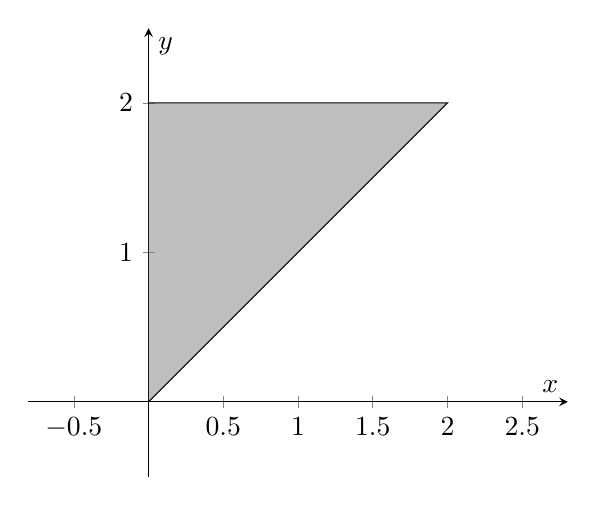
\begin{tikzpicture}
                \begin{axis}[
                    axis lines = center,
                    xlabel = $x$,
                    ylabel = $y$,
                    xmin = -0.5, xmax = 2.5,
                    ymin = -0.5, ymax = 2.5,
                    legend pos = north west,
                    axis equal,
                ]
                    % Triángulo (0,0) (2,2) (0,2)
                    \addplot[fill=gray, fill opacity=0.5] coordinates {(0,0) (2,2) (0,2)};
                \end{axis}
            \end{tikzpicture}
        \end{figure}

        Como la función de densidad es constante, tenemos que:
        \begin{equation*}
            f_{(X,Y)}(x, y) = \begin{cases}
                k, & (x, y) \in T \\
                0, & \text{en otro caso}
            \end{cases}
        \end{equation*}

        Para calcular $k$, tenemos que:
        \begin{align*}
            1 &= \int_{T} f_{(X,Y)} = \int_T k = k\lm(T) = k\cdot 2
            \Longrightarrow k=\nicefrac{1}{2}
        \end{align*}
        \item Curvas y rectas de regresión de $X$ sobre $Y$ y de $Y$ sobre $X$.
        
        Comenzamos calculando las curvas de regresión, ya que si estas son funciones lineales, las rectas de regresión coincidirán con las curvas de regresión.
        Para ello, calculamos las funciones de densidad marginales y condicionadas.
        \begin{itemize}
            \item Función de densidad de $X$. Para $x\in \left]0,2\right[$:
            \begin{align*}
                f_X(x) &= \int_{-\infty}^{\infty} f_{(X,Y)}(x, y) \ dy
                = \int_{x}^{2} \nicefrac{1}{2} \ dy = \nicefrac{1}{2}(2-x)
                = 1-\frac{x}{2}
            \end{align*}

            \item Función de densidad de $Y$. Para $y\in \left]0,2\right[$:
            \begin{align*}
                f_Y(y) &= \int_{-\infty}^{\infty} f_{(X,Y)}(x, y) \ dx
                = \int_{0}^{y} \nicefrac{1}{2} \ dx = \frac{y}{2}
            \end{align*}

            \item Función de densidad condicionada de $X$ dado $Y=y^*\in \left]0,2\right[$. Para $x\in \left]0,y^*\right[$:
            \begin{align*}
                f_{X\mid Y=y^*}(x) &= \dfrac{f_{(X,Y)}(x, y^*)}{f_Y(y^*)}
                = \dfrac{\nicefrac{1}{2}}{\nicefrac{y^*}{2}}
                = \dfrac{1}{y^*}
            \end{align*}

            \item Función de densidad condicionada de $Y$ dado $X=x^*\in \left]0,2\right[$. Para $y\in \left]x^*,2\right[$:
            \begin{align*}
                f_{Y\mid X=x^*}(y) &= \dfrac{f_{(X,Y)}(x^*, y)}{f_X(x^*)}
                = \dfrac{\nicefrac{1}{2}}{1-\nicefrac{x^*}{2}}
                = \dfrac{1}{2-x^*}
            \end{align*}
        \end{itemize}

        Calculamos ahora las curvas de regresión.
        \begin{itemize}
            \item Curva de regresión de $X$ sobre $Y$:
            \begin{align*}
                \wh{X}(y) &= E[X\mid Y = y] = \int_{0}^{y} x f_{X\mid Y=y}(x) \ dx
                = \int_{0}^{y} x\cdot  \dfrac{1}{y} \ dx
                = \dfrac{1}{y} \int_{0}^{y} x \ dx
                =\\&= \dfrac{1}{y} \left[\dfrac{x^2}{2}\right]_{0}^{y}
                = \dfrac{y}{2} \qquad \forall y\in \left]0,2\right[
            \end{align*}

            \item Curva de regresión de $Y$ sobre $X$:
            \begin{align*}
                \wh{Y}(x) &= E[Y\mid X = x] = \int_{x}^{2} y f_{Y\mid X=x}(y) \ dy
                = \int_{x}^{2} y\cdot  \dfrac{1}{2-x} \ dy
                = \dfrac{1}{2-x} \int_{x}^{2} y \ dy
                =\\&= \dfrac{1}{2-x} \left[\dfrac{y^2}{2}\right]_{x}^{2}
                = \dfrac{2^2 - x^2}{2(2-x)}
                = \dfrac{4-x^2}{2(2-x)}
                = \dfrac{2+x}{2} = 1 + \dfrac{x}{2} \qquad \forall x\in \left]0,2\right[
            \end{align*}
        \end{itemize}

        Tenemos además que las curvas de regresión son funciones lineales, por lo que las rectas de regresión coinciden con las curvas de regresión.
        \item Razones de correlación y coeficiente de correlación lineal.
        
        Como las curvas de regresión son funciones lineales, tenemos que las razones de correlación coinciden y son iguales al coeficiente de determinación lineal.
        \begin{equation*}
            \eta_{Y/X}^2 = \eta_{X/Y}^2 = \rho_{Y/X}^2 = \dfrac{\Cov[X,Y]^2}{\Var[X]\Var[Y]}
        \end{equation*}
        
        Como este es el producto de las pendientes de las rectas de regresión, tenemos que:
        \begin{equation*}
            \rho_{Y/X}^2 = \dfrac{1}{2}\cdot \dfrac{1}{2} = \dfrac{1}{4}
        \end{equation*}

        Como la correlación es positiva por ser ambas rectas crecientes, tenemos que:
        \begin{equation*}
            \rho_{Y/X} =  + \sqrt{\rho_{Y/X}^2} = \nicefrac{1}{2}
        \end{equation*}

        \item Error cuadrático medio asociado a cada una de las funciones de regresión.
        
        Por lo visto en teoría, sabemos que:
        \begin{align*}
            \text{ECM}(\wh{X}) &= \Var[X] - \dfrac{\Cov[X,Y]^2}{\Var[Y]}\\
            \text{ECM}(\wh{Y}) &= \Var[Y] - \dfrac{\Cov[X,Y]^2}{\Var[X]}
        \end{align*}

        Calculamos por tanto los valores necesarios:
        \begin{align*}
            E[X] &= \int_{0}^{2} x f_X(x) \ dx = \int_{0}^{2} x(1-\nicefrac{x}{2}) \ dx
            = \left[\dfrac{x^2}{2} - \dfrac{x^3}{6}\right]_{0}^{2}
            = \dfrac{4}{2} - \dfrac{8}{6} = \dfrac{2}{3}\\
            E[Y] &= \int_{0}^{2} y f_Y(y) \ dy = \int_{0}^{2} y\cdot \nicefrac{y}{2} \ dy
            = \left[\dfrac{y^3}{6}\right]_{0}^{2} = \dfrac{8}{6} = \frac{4}{3}\\
            E[X^2] &= \int_{0}^{2} x^2 f_X(x) \ dx = \int_{0}^{2} x^2(1-\nicefrac{x}{2}) \ dx
            = \left[\dfrac{x^3}{3} - \dfrac{x^4}{8}\right]_{0}^{2}
            = \dfrac{8}{3} - \dfrac{16}{8} = \dfrac{2}{3}\\
            E[Y^2] &= \int_{0}^{2} y^2 f_Y(y) \ dy = \int_{0}^{2} y^2\cdot \nicefrac{y}{2} \ dy
            = \left[\dfrac{y^4}{8}\right]_{0}^{2} = \dfrac{16}{8} = 2\\
            E[XY] &= \int_{0}^{2} \int_{x}^{2} xy f_{(X,Y)}(x, y) \ dy \ dx
            = \int_{0}^{2} \int_{x}^{2} xy\cdot \nicefrac{1}{2} \ dy \ dx
            = \frac{1}{2} \int_{0}^{2} x\left[\dfrac{y^2}{2}\right]_{x}^{2} \ dx
            =\\&= \frac{1}{4} \int_{0}^{2} x\left(4 - x^2\right) \ dx
            = \frac{1}{4} \left[2x^2 - \frac{x^4}{4}\right]_{0}^{2}
            = \frac{1}{4} \left(8 - 4\right) = 1\\
            \Var[X] &= E[X^2] - E[X]^2 = \frac{2}{3} - \left(\frac{2}{3}\right)^2 = \frac{2}{9}\\
            \Var[Y] &= E[Y^2] - E[Y]^2 = 2 - \left(\frac{4}{3}\right)^2 = \frac{2}{9}\\
            \Cov[X,Y] &= E[XY] - E[X]E[Y] = 1 - \frac{2}{3}\cdot \frac{4}{3} = \frac{1}{9}
        \end{align*}

        Por tanto, tenemos que:
        \begin{align*}
            \text{ECM}(\wh{X}) &= \Var[X] - \dfrac{\Cov[X,Y]^2}{\Var[Y]}
            = \frac{2}{9} - \dfrac{\nicefrac{1}{9}^2}{\nicefrac{2}{9}}
            = \frac{2}{9} - \frac{1}{18} = \frac{3}{18} = \frac{1}{6}\\
            \text{ECM}(\wh{Y}) &= \Var[Y] - \dfrac{\Cov[X,Y]^2}{\Var[X]}
            = \frac{2}{9} - \dfrac{\nicefrac{1}{9}^2}{\nicefrac{2}{9}}
            = \frac{2}{9} - \frac{1}{18} = \frac{3}{18} = \frac{1}{6}
        \end{align*}
    \end{enumerate}
\end{ejercicio}

\begin{ejercicio}
    Dada la función masa de probabilidad del vector aleatorio $(X,Y)$
    \begin{equation*}
        \begin{array}{c|cccc||c}
            X\setminus Y & 0 & 1 & 2 & 3\\
            \hline
            0 & 0.2 & 0.2 & 0.05 & 0 & 0.45\\
            1 & 0.1 & 0.1 & 0.1 & 0.05 & 0.35\\
            2 & 0 & 0.05 & 0.05 & 0.1 & 0.2\\
            \hline \hline
            & 0.3 & 0.35 & 0.2 & 0.15 & 1
        \end{array}
    \end{equation*}
    \begin{enumerate}
        \item Determinar la aproximación lineal mínimo cuadrática de $Y$ para $X = 1$.
        
        Nos piden la recta de regresión de $Y$ sobre $X$, y evaluarla en el punto $X=1$.
        Calculamos las esperanzas necesarias para el cálculo de la recta de regresión.
        \begin{align*}
            E[X] &= 0\cdot 0.3 + 1\cdot 0.35 + 2\cdot 0.2 = 0.75\\
            E[Y] &= 0\cdot 0.3 + 1\cdot 0.35 + 2\cdot 0.2 + 3\cdot 0.15 = 1.2\\
            E[X^2] &= 0^2\cdot 0.3 + 1^2\cdot 0.35 + 2^2\cdot 0.2 = 1.15\\
            E[XY] &= \sum_{\substack{x\in E_X\\y\in E_Y}}xyP[X = x, Y = y] = 1.35\\
            \Var[X] &= E[X^2] - E[X]^2 = 1.15 - 0.75^2 = 0.5875\\
            \Cov[X,Y] &= E[XY] - E[X]E[Y] = 1.35 - 0.75\cdot 1.2 = 0.45
        \end{align*}

        Calculamos ahora la recta de regresión de $Y$ sobre $X$.
        \begin{align*}
            \wh{Y}(x) &= E[Y] + \dfrac{\Cov[X,Y]}{\Var[X]}(x - E[X])
            = 1.2 + \dfrac{0.45}{0.5875}(x - 0.75)
            = 1.2 + \dfrac{36}{47}(x - 0.75)
        \end{align*}

        Evaluando en $X=1$, tenemos que:
        \begin{equation*}
            \wh{Y}(1) = 1.2 + \dfrac{36}{47}(1 - 0.75) = 1.2 + \dfrac{36}{47}\cdot 0.25 = 1.2 + \dfrac{9}{47} \approx 1.391489
        \end{equation*}
        \item Determinar la aproximación mínimo cuadrática de $Y$ para $X = 1$.
        
        En este caso, piden $E[Y\mid X = 1]$. Para ello, hemos de calcular las distribución condicionada de $Y$ dado $X = 1$.
        \begin{align*}
            P[Y = 0\mid X = 1] &= \dfrac{P[X = 1, Y = 0]}{P[X = 1]} = \dfrac{0.1}{0.35} = \frac{2}{7}\\
            P[Y = 1\mid X = 1] &= \dfrac{P[X = 1, Y = 1]}{P[X = 1]} = \dfrac{0.1}{0.35} = \frac{2}{7}\\
            P[Y = 2\mid X = 1] &= \dfrac{P[X = 1, Y = 2]}{P[X = 1]} = \dfrac{0.1}{0.35} = \frac{2}{7}\\
            P[Y = 3\mid X = 1] &= \dfrac{P[X = 1, Y = 3]}{P[X = 1]} = \dfrac{0.05}{0.35} = \frac{1}{7}
        \end{align*}

        Por tanto, tenemos que:
        \begin{align*}
            E[Y\mid X = 1] &= \sum_{y\in E_Y} y P[Y = y\mid X = 1] =\\&= 0+1\cdot P[Y = 1\mid X = 1] + 2\cdot P[Y = 2\mid X = 1] + 3\cdot P[Y = 3\mid X = 1]
            =\\&= \dfrac{2}{7} + 2\cdot \dfrac{2}{7} + 3\cdot \dfrac{1}{7} = \dfrac{9}{7}
        \end{align*}
    \end{enumerate}
\end{ejercicio}

\begin{ejercicio}
    Dadas las siguientes distribuciones, determinar qué variable, $X$ ó $X'$, aproxima mejor a la variable $Y$:
    \begin{equation*}
        \begin{array}{c|ccc||c}
            X\setminus Y & 0 & 1 & 2\\
            \hline
            0 & \nicefrac{1}{5} & 0 & 0 & \nicefrac{1}{5}\\
            2 & 0 & \nicefrac{1}{5} & 0 & \nicefrac{1}{5}\\
            3 & \nicefrac{1}{5} & 0 & \nicefrac{1}{5} & \nicefrac{2}{5}\\
            4 & 0 & 0 & \nicefrac{1}{5} & \nicefrac{1}{5}\\
            \hline \hline
            & \nicefrac{2}{5} & \nicefrac{1}{5} & \nicefrac{2}{5} & 1
        \end{array}
        \hspace{2cm}
        \begin{array}{c|ccc||c}
            X'\setminus Y & 0 & 1 & 2\\
            \hline
            0 & \nicefrac{1}{5} & 0 & \nicefrac{1}{5} & \nicefrac{2}{5}\\
            2 & 0 & \nicefrac{1}{5} & 0 & \nicefrac{1}{5}\\
            3 & \nicefrac{1}{5} & 0 & 0 & \nicefrac{1}{5}\\
            4 & 0 & 0 & \nicefrac{1}{5} & \nicefrac{1}{5}\\
            \hline \hline
            & \nicefrac{2}{5} & \nicefrac{1}{5} & \nicefrac{2}{5} & 1
        \end{array}
    \end{equation*}

    Hemos de obtener $\eta^2_{Y/X}$ y $\eta^2_{Y/X'}$ para compararlas.
    \begin{equation*}
        \eta^2_{Y/X} = \dfrac{\Var[E[Y\mid X]]}{\Var[Y]}, \qquad \eta^2_{Y/X'} = \dfrac{\Var[E[Y\mid X']]}{\Var[Y]}
    \end{equation*}

    Calculamos las esperanzas necesarias para el cálculo de las varianzas.
    \begin{align*}
        E[Y] &= 0\cdot \nicefrac{2}{5} + 1\cdot \nicefrac{1}{5} + 2\cdot \nicefrac{2}{5} = 1\\
        E[Y^2] &= 0^2\cdot \nicefrac{2}{5} + 1^2\cdot \nicefrac{1}{5} + 2^2\cdot \nicefrac{2}{5} = \nicefrac{9}{5}\\
        E[E[Y\mid X]] &= E[Y] = 1\\
        E[E[Y\mid X']] &= E[Y] = 1 \\
        E[(E[Y\mid X])^2] &= \sum_{x\in E_X} (E[Y\mid X = x])^2 P[X = x]\\
        E[(E[Y\mid X'])^2] &= \sum_{x\in E_{X'}} (E[Y\mid X' = x])^2 P[X' = x]
    \end{align*}

    Calculamos por tanto las esperanzas condicionadas.
    \begin{align*}
        E[Y\mid X = 0] &= 0\cdot 1 + 1\cdot 0 + 2\cdot 0 = 0\\
        E[Y\mid X = 2] &= 0\cdot 0 + 1\cdot 1 + 2\cdot 0 = 1\\
        E[Y\mid X = 3] &= 0\cdot \nicefrac{1}{2} + 1\cdot 0 + 2\cdot \nicefrac{1}{2} = 1\\
        E[Y\mid X = 4] &= 0\cdot 0 + 1\cdot 0 + 2\cdot 1 = 2\\
        E[Y\mid X' = 0] &= 0\cdot \nicefrac{1}{2} + 1\cdot 0 + 2\cdot \nicefrac{1}{2} = 1\\
        E[Y\mid X' = 2] &= 0\cdot 0 + 1\cdot 1 + 2\cdot 0 = 1\\
        E[Y\mid X' = 3] &= 0\cdot \nicefrac{1}{2} + 1\cdot 0 + 2\cdot \nicefrac{1}{2} = 1\\
        E[Y\mid X' = 4] &= 0\cdot 0 + 1\cdot 0 + 2\cdot 1 = 2
    \end{align*}

    Por tanto, hemos comprobado que $E[Y\mid X] = E[Y\mid X']$, por lo que:
    \begin{equation*}
        E[Y\mid X]=E[Y\mid X'] \Longrightarrow
        \Var[E[Y\mid X]] = \Var[E[Y\mid X']]
        \Longrightarrow \eta^2_{Y/X} = \eta^2_{Y/X'}
    \end{equation*}

    Por tanto, ambas variables aproximan igual de bien a $Y$. Veamos cómo es la aproximación calculando aun así los coeficientes. Tenemos que:
    \begin{align*}
        E[(E[Y\mid X])^2] &= \sum_{x\in E_X} (E[Y\mid X = x])^2 P[X = x]
        =\\&= 0^2\cdot \nicefrac{1}{5} + 1^2\cdot \nicefrac{1}{5} + 1^2\cdot \nicefrac{2}{5} + 2^2\cdot \nicefrac{1}{5} = \nicefrac{7}{5}
    \end{align*}

    Por tanto, tenemos que:
    \begin{align*}
        \Var[Y] = E[Y^2] - E[Y]^2 = \nicefrac{9}{5} - 1 = \nicefrac{4}{5}\\
        \Var[E[Y\mid X]] = E[(E[Y\mid X])^2] - E[E[Y\mid X]]^2 = \nicefrac{7}{5} - 1 = \nicefrac{2}{5}
    \end{align*}

    Por tanto, tenemos que:
    \begin{equation*}
        \eta^2_{Y/X} = \dfrac{\Var[E[Y\mid X]]}{\Var[Y]} = \dfrac{\nicefrac{2}{5}}{\nicefrac{4}{5}} = \nicefrac{1}{2} = \eta^2_{Y/X'}
    \end{equation*}

    Por tanto, tenemos que ninguno de los ajustes es bueno, ya que solo explican la mitad de la variabilidad de $Y$.
\end{ejercicio}

\begin{ejercicio} \label{ej:4.7}
    Probar que las variables $X = U + V$ e $Y = U - V$ son incorreladas, pero no independientes, si $U$ y $V$ son variables aleatorias con función de densidad conjunta:
    \begin{equation*}
        f_{U,V}(u, v) = \exp(-u-v), \quad u, v > 0.
    \end{equation*}

    % // TODO: Incorreladas?
    % Es la forma más fácil

    Veamos que no son independientes. Para ello, calculamos en primer lugar $f_{X,Y}(x, y)$. Para ello, definimos la transformación:
    \Func{g}{\mathbb{R}^2}{\mathbb{R}^2}{(U,V)}{(X,Y)=(U+V,U-V)}

    Para obtener $g^{-1}$, buscamos obtener $U,V$ en función de $X,T$:
    \begin{equation*}
        \left\{
            \begin{aligned}
                X=U+V\\
                Y=U-V
            \end{aligned}
        \right\}
        \Longrightarrow
        \left\{
            \begin{aligned}
                U=\nicefrac{X+Y}{2}\\
                V=\nicefrac{X-Y}{2}
            \end{aligned}
        \right\}
    \end{equation*}

    Por tanto, tenemos que $\exists g^{-1}$, con:
    \Func{g^{-1}}{\mathbb{R}^2}{\mathbb{R}^2}{(X,Y)}{(U,V)=\left(\frac{X+Y}{2},\frac{X-Y}{2}\right)}

    Tenemos que todas las componentes de $g^{-1}$ son derivables:
    \begin{align*}
        \dfrac{\partial U}{\partial X} &= \dfrac{1}{2}, & \dfrac{\partial U}{\partial Y} &= \dfrac{1}{2}, & \dfrac{\partial V}{\partial X} &= \dfrac{1}{2}, & \dfrac{\partial V}{\partial Y} &= -\dfrac{1}{2}
    \end{align*}

    Además, veamos que el jacobianos no se anula:
    \begin{equation*}
        \det Jg^{-1}(x,y)=\begin{vmatrix}
            \nicefrac{1}{2} & \nicefrac{1}{2}\\
            \nicefrac{1}{2} & \nicefrac{-1}{2}
        \end{vmatrix}=
        \dfrac{1}{2^2}\cdot \begin{vmatrix}
            1 & 1\\
            1 & -1
        \end{vmatrix}=
        -\frac{1}{2}\neq 0 \qquad \forall (x,y)\in\bb{R}^2.
    \end{equation*}

    Por tanto, podemos aplicar el teorema del cambio de variable para obtener $f_{X,Y}(x,y)$:
    \begin{align*}
        f_{X,Y}(x,y) &= f_{U,V}(g^{-1}(x,y))\cdot |Jg^{-1}(x,y)|
        = \dfrac{1}{2}\cdot f_{U,V}\left(\frac{x+y}{2},\frac{x-y}{2}\right)\\
        &= \dfrac{1}{2}\cdot \exp\left(-\frac{x+y}{2}-\frac{x-y}{2}\right)
        = \dfrac{1}{2}\cdot \exp\left(\dfrac{-x-y-x+y}{2}\right)
        =\\&= \dfrac{1}{2}\cdot \exp\left(-x\right)
        \qquad \forall (x,y)\in \bb{R}^2 \text{ tal que } x+y, x-y>0
    \end{align*}

    Veamos el conjunto gráficamente:
    \begin{figure}[H]
        \centering
        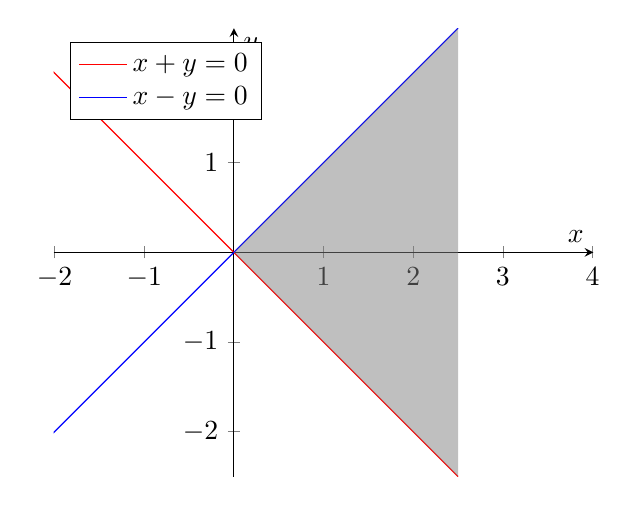
\begin{tikzpicture}
            \begin{axis}[
                axis lines = center,
                xlabel = $x$,
                ylabel = $y$,
                xmin = -0.5, xmax = 2.5,
                ymin = -2.5, ymax = 2.5,
                legend pos = north west,
                axis equal,
            ]
                % Recta x+y=0
                \addplot[domain=-5:2.5, samples=2, color=red]{-x};
                \addlegendentry{$x+y=0$}

                % Recta x-y=0
                \addplot[domain=-5:2.5, samples=2, color=blue]{x};
                \addlegendentry{$x-y=0$}

                % triangulo (0,0) (5,5) (5,-5)
                \addplot[fill=gray, fill opacity=0.5, draw=none] coordinates {(0,0) (2.5,2.5) (2.5,-2.5)};
            \end{axis}
        \end{tikzpicture}
    \end{figure}

    Tenemos que el conjunto donde $f_{X,Y}(x,y)$ no se puede expresar como producto cartesiano, por lo que intuimos que $X$ e $Y$ no son independientes. Para comprobarlo, calculamos la función de densidad marginal de $X$ y $Y$:
    \begin{align*}
        f_X(x) &= \int_{-\infty}^{\infty} f_{X,Y}(x, y) \ dy
        = \int_{-x}^{x} \nicefrac{1}{2}\exp(-x) \ dy
        = \nicefrac{1}{2}\exp(-x)\left[y\right]_{-x}^{x}
        =\\&= \nicefrac{1}{2}\exp(-x)(x+x) = xe^{-x} \qquad \forall x>0
    \end{align*}

    Para calcular la marginal de $Y$, distinguimos en función de $y$:
    \begin{itemize}
        \item Si $y>0$:
        \begin{align*}
            f_Y(y) &= \int_{-\infty}^{\infty} f_{X,Y}(x, y) \ dx
            = \int_{y}^{\infty} \nicefrac{1}{2}\exp(-x) \ dx
            = \nicefrac{1}{2}\left[-\exp(-x)\right]_{y}^{\infty}
            =\\&= \nicefrac{1}{2}\left[0 - (-\exp(-y))\right]
            = \frac{e^{-y}}{2} \qquad \forall y>0
        \end{align*}

        \item Si $y\leq 0$:
        \begin{align*}
            f_Y(y) &= \int_{-\infty}^{\infty} f_{X,Y}(x, y) \ dx
            = \int_{-y}^{\infty} \nicefrac{1}{2}\exp(-x) \ dx
            = \nicefrac{1}{2}\left[-\exp(-x)\right]_{-y}^{\infty}
            =\\&= \nicefrac{1}{2}\left[0 - (-\exp(y))\right]
            = \frac{e^{y}}{2} \qquad \forall y\leq 0
        \end{align*}
    \end{itemize}

    Por tanto, tenemos que:
    \begin{align*}
        f_Y(y)=\begin{cases}
            \dfrac{e^{-y}}{2} & y>0\\ \\
            \dfrac{e^{y}}{2} & y\leq 0
        \end{cases}
    \end{align*}

    Para el $(1,1)$, tenemos que:
    \begin{align*}
        f_X(1) &= e^{-1}, & f_{X,Y}(1,1)=\frac{1}{2}e^{-1} \\
        f_Y(1) &= \frac{1}{2}e^{-1} 
    \end{align*}

    Por tanto, no se cumple que $f_{X,Y}(x,y)=f_X(x)f_Y(y)$ para todo $(x,y)\in\bb{R}^2$, por lo que $X$ e $Y$ no son independientes.
\end{ejercicio}

\begin{ejercicio}
    % // TODO: Hacer
    Sea $X$ una variable aleatoria con distribución uniforme en el intervalo $[0,1]$, y sea $Y$ una variable aleatoria continua tal que
    \begin{equation*}
        f_{Y\mid X=x}(y) = \begin{cases}
            \nicefrac{1}{x^2} & y \in \left[0, x^2\right]\\
            0 & \text{en caso contrario}
        \end{cases}
    \end{equation*}
    \begin{enumerate}
        \item\label{ej:4.8.a} Calcular la función de densidad de probabilidad conjunta de $X$ e $Y$. Calcular la función de densidad de probabilidad marginal de $Y$.
        \item Calcular $E[X\mid Y = y]$ y $E[Y\mid X = x]$.
        \item Para la misma densidad de probabilidad condicionada del apartado \ref{ej:4.8.a}, considerando ahora que $X$ es una variable aleatoria continua con función de densidad de probabilidad:
        \begin{equation*}
            f_X(x) = \begin{cases}
                3x^2 & x \in \left[0,1\right]\\
                0 & \text{en caso contrario}
            \end{cases}
        \end{equation*}
        Calcular de nuevo la función de densidad de probabilidad conjunta de $X$ e $Y$, y la función de densidad de probabilidad marginal de $Y$, así como $E[X\mid Y = y]$ y $E[Y\mid X = x]$.
    \end{enumerate}
\end{ejercicio}

\begin{ejercicio}
    Sean $X$ e $Y$ variables aleatorias con función de densidad conjunta:
    \begin{equation*}
        f_{(X,Y)}(x, y) = \begin{cases}
            x+y & (x, y) \in [0,1] \times [0,1]\\
            0 & \text{en caso contrario}
        \end{cases}
    \end{equation*}
    \begin{enumerate}
        \item Calcular la predicción mínimo cuadrática de $Y$ a partir de $X$ y el error cuadrático medio asociado.
        \item Si se observa $X = \nicefrac{1}{2}$, qué predicción de $Y$ tiene menor error cuadrático medio? Calcular dicho error.
        \item Supóngase que una persona debe pagar una cantidad $C$ por la oportunidad de observar el valor de $X$ antes de predecir el valor de $Y$, o puede simplemente predecir el valor de $Y$ sin observar $X$. Si la persona considera que su pérdida total es la suma de $C$ y el error cuadrático medio de su predicción, qué valor máximo de $C$ estaría dispuesta a pagar?
    \end{enumerate}
\end{ejercicio}

\begin{ejercicio}
    Sea $(X,Y)$ un vector aleatorio con función de densidad:
    \begin{equation*}
        f_{(X,Y)}(x, y) = \exp(-y), \quad 0 < x < y
    \end{equation*}
    Obtener y representar las rectas y curvas de regresión. Calcular el coeficiente de correlación lineal, las razones de correlación y el error cuadrático medio cometido al predecir cada variable según cada una de las funciones de regresión. Interpretar los resultados.
\end{ejercicio}

\begin{ejercicio}
    Sea $(X,Y)$ un vector aleatorio con función de densidad uniforme sobre el cuadrado unidad. Obtener y representar las rectas y curvas de regresión. Calcular el coeficiente de correlación lineal, las razones de correlación y el error cuadrático medio cometido al predecir cada variable según cada una de las funciones de regresión. Interpretar los resultados.
\end{ejercicio}

\begin{ejercicio}
    Supongamos que $(X,Y)$ tiene función de densidad de probabilidad conjunta dada por:
    \begin{equation*}
        f_{(X,Y)}(x, y) = \begin{cases}
            1, & |y| < x, x \in \left]0,1\right[\\
            0, & \text{en otro caso}
        \end{cases}
    \end{equation*}
    Obtener y representar las rectas y curvas de regresión. Calcular el coeficiente de correlación lineal, las razones de correlación y el error cuadrático medio cometido al predecir cada variable según cada una de las funciones de regresión. Interpretar los resultados.
\end{ejercicio}

\begin{ejercicio}
    Sea $(X,Y)$ un vector aleatorio distribuido uniformemente en el paralelogramo de vértices $(0,0)$; $(2,0)$; $(3,1)$ y $(1,1)$. Calcular el error cuadrático medio asociado a la predicción de $X$ a partir de la variable $Y$ y a la predicción de $Y$ a partir de la variable aleatoria $X$. Determinar la predicción más fiable a la vista de los resultados obtenidos.
\end{ejercicio}

\begin{ejercicio}
    Sea $(X,Y)$ un vector aleatorio con rectas de regresión
    \begin{equation*}
        x+4y = 1 \qquad x+5y = 2
    \end{equation*}
    \begin{enumerate}
        \item Cuál es la recta de regresión de $Y$ sobre $X$?
        \item Calcular el coeficiente de correlación lineal y la proporción de varianza de cada variable que queda explicada por la regresión lineal.
        \item Calcular las medias de ambas variables
    \end{enumerate}
\end{ejercicio}